\chapter{Revisão bibliográfica}
\label{Revisão bibliográfica}

Neste Capítulo, exploramos a aplicação de redes neurais profundas na avaliação da função cardíaca utilizando vídeos de ecocardiograma, com o objetivo de analisar e discutir trabalhos relevantes nesse campo.  A Seção \ref{Revisão Sistemática da Literatura} descreve a metodologia de Revisão Sistemática da Literatura (SLR), onde apresentamos uma visão geral das estratégias utilizadas para a seleção dos trabalhos pertinentes. Na Seção \ref{Estudos selecionados} descreve os aspectos teóricos das redes neurais profundas empregadas nos estudos escolhidos, seguidos por uma apresentação e discussão criteriosa dos trabalhos relacionados a essa redes neurais, organizados por temas relevantes para a área de interesse deste trabalho. Esta Seção é estruturada de forma a proporcionar um aprofundamento teórico nas tecnologias de redes neurais, enquanto simultaneamente contextualiza cada estudo selecionado dentro do âmbito da avaliação da função cardíaca por meio de ecocardiograma.
 Em cada bloco temático desta Seção, após a apresentação dos trabalhos, incluímos uma discussão detalhada, examinando a metodologia, os resultados e as contribuições de cada pesquisa para o campo da avaliação cardíaca. Essas discussões são integradas ao final de cada tema, proporcionando uma análise abrangente que destaca tanto os avanços técnicos quanto as implicações práticas desses estudos no contexto mais amplo da avaliação cardíaca utilizando tecnologias de aprendizado profundo. Através desta abordagem, o Capítulo oferece uma perspectiva completa sobre como as redes neurais profundas estão sendo utilizadas para inovar e melhorar a precisão da avaliação cardíaca em ecocardiogramas.

\section{Revisão Sistemática da Literatura}
\label{Revisão Sistemática da Literatura}

O protocolo de revisão sistemática da literatura, estabelecido seguindo as orientações de \cite{kitchenham2009systematic}, é um estudo que tem como objetivo fornecer uma abordagem imparcial, objetiva e sistemática para responder a questões específicas de pesquisa, tópicos de uma área ou fenômenos de interesse. Esses fenômenos, conhecidos como estudos primários, são analisados e sintetizados dentro do contexto da revisão, permitindo uma compreensão aprofundada e estruturada do campo em questão.

A Revisão Sistemática da Literatura (SLR) constitui um método meticuloso e estruturado, essencial para compreender as tendências e os avanços em campos específicos, como a avaliação de imagens e vídeos de ecocardiograma usando abordagens de Deep Learning. Este método, pautado pelas diretrizes de \textcite{kitchenham2009systematic}, divide-se em três fases fundamentais: planejamento, condução e relatório. Na fase de planejamento, a ênfase recai sobre a definição clara das questões de pesquisa. Este passo é crucial pois as questões moldam o escopo da revisão, direcionando a busca e análise dos estudos. As questões devem ser precisas e relevantes, refletindo as necessidades de informação no campo de estudo. A formulação destas questões é descrita na Seção \ref{Questões de pesquisa} e serve como a espinha dorsal para as etapas subsequentes. Seguindo para a fase de condução, detalhada na Seção \ref{Abordagem de pesquisa}, o processo se volta para a identificação e seleção de estudos relevantes. Esta etapa é caracterizada por uma busca sistemática em bases de dados e literatura científica, utilizando critérios de inclusão e exclusão. A condução é uma fase detalhada, garantindo que apenas os estudos mais pertinentes e de alta qualidade sejam considerados para análise. Por fim, a fase de relatório trata da síntese e apresentação dos resultados encontrados. Aqui, os estudos selecionados são avaliados, analisados e os achados são relatados de maneira estruturada e coerente. A qualidade dos estudos incluídos é avaliada, conforme descrito na subSeção \ref{Avaliação de qualidade}.

\subsection{Questões de pesquisa}
\label{Questões de pesquisa}

Esta revisão sistemática da literatura teve como objetivo apresentar os estudos que foram publicados na área de avaliação de imagens e vídeos de ecocardiograma  usando abordagens de \textit{Deep Learning} . As questões de pesquisa abordadas por esta pesquisa são:

Questão 1 (Q1) Em quais tipos de ecocardiograma a IA foi aplicada ?

Questão 2 (Q2) - Quais estruturas do coração o artigo trata?

Questão 3 (Q3) - Quais marcadores ou doença são avaliado?

Questão 4 (Q4) - Quais modelos de \textit{Machine Learning}  ou \textit{Deep Learning}  vêm sendo mais utilizados para avaliação do coração?

Questão 5 (Q5) - Quais conjuntos de dados são utilizadas para treinar e testar os algoritmos de \textit{Machine Learning}/\textit{Deep Learning} ?

Questão 6 (Q6) - Quais são os parâmetros de avaliação e abordagens utilizadas para modelos de DL/ML  em ecocardiograma foi aplicada para apoiar a decisão médica?

\subsection {Abordagem de pesquisa}
\label{Abordagem de pesquisa}

Uma abordagem sistemática foi adotada para restringir os resultados da pesquisa aos artigos que estão diretamente relacionados ao escopo do SLR. Para identificar contribuições relacionadas, motores de busca como Science Direct , IEEE Explore, PubMed  e Google Scholar foram consultados para artigos contendo (“machine learning” OR “deep learning”) AND (“Echocardiography”)  no título e resumo. 

A última atualização dos documentos incluídos foi em 1º de setembro de 2022.

Todos os resultados foram processados e as strings de busca acima mencionadas resultaram em um total de 436 estudos.

\subsection {Critério de seleção}
\label{Critério de seleção}

Nesta etapa serão definidos os critérios de seleção/inclusão e exclusão para definir quais artigos passarão para a próxima etapa da revisão. Os critérios devem ser definidos a partir das questões de pesquisa. Os resultados da pesquisa de diferentes bancos de dados foram adicionados a uma planilha e verificados de acordo com os critérios de seleção. Para que um estudo seja incluído, todos os critérios de inclusão devem ser verdadeiros e os critérios de exclusão devem ser falsos \cite{kitchenham2009systematic}.

Todos os estudos extraídos que pudessem responder às questões de pesquisa foram considerados potencialmente relevantes e selecionados para passar pelos critérios de inclusão e exclusão apresentados a seguir.

A publicação é sobre o uso de Deep Learning ou Machine Learning para análises de vídeos e imagens em ecocardiograma. 

A publicação é um estudo primário. (Estudos primários são investigações originais que envolvem a coleta e análise de dados diretamente dos experimentos ou observações, sem depender de dados já publicados por outros estudos. Eles são a fonte principal de novas informações científicas.)

O artigo foi publicado após o ano de 2019. 

Os critérios de exclusão utilizados foram os seguintes.

1: A publicação não está relacionada ao Deep Learning ou Machine learning para  analises de vídeos e imagens em ecocardiograma.

2: A publicação é duplicada ou recuperada de outro banco de dados.

3: O texto completo do estudo não está disponível.

4: O estudo não está publicado na língua inglesa


Após a exclusão dos registros duplicados (n = 32), os critérios de seleção foram aplicados aos demais registros (n = 404). Assim, um total de 113 artigos de texto completo foram avaliados para elegibilidade. Para a seleção dos artigos finais, foram considerados artigos publicados nos últimos três anos. 

\subsection {Avaliação de qualidade}
\label{Avaliação de qualidade}

O próximo passo no protocolo de revisão foi a execução da  avaliação da qualidade. \textcite{kitchenham2009systematic} define que esse passo tem como objetivo avaliar melhor os estudos incluídos e remover estudos que não se encaixam no objetivo desta revisão ou que não descrevem os detalhes que são importantes para esta revisão com detalhes suficientes. 

Com esse objetivo, foram estabelecidos os  seguintes critérios de avaliação:

1: O objetivo da pesquisa está claramente descrito?

2: O artigo possui citações? Se sim são citações é > 5 ou > 15?

3: Os autores descreveram as limitações do estudo?

4: O estudo deixa claro quais foram as oportunidades identificadas?

5: O estudo conseguiu resolver o ou propor solução para o problema proposto?

Para execução desta etapa, os artigos foram analisados para responder aos critérios de avaliações propostos. pode ser obtido 1 ponto se o critério for atendido, ou meio ponto se for parcialmente atendido. Isso deu uma pontuação de qualidade entre 0 e 5 para cada estudo. Artigos com pontuação acima ou iguais a 4,5 foram incluídos nesta revisão.

O fluxograma das etapas iterativas de seleção dos estudos foi elaborado a partir
da metodologia e está apresentado na Figura \ref{fig:fluxoslr}. A Tabela \ref{tab:trabalhos} apresenta os artigos selecionados para leitura na íntegra.

\begin{figure}[H]
   \centering
   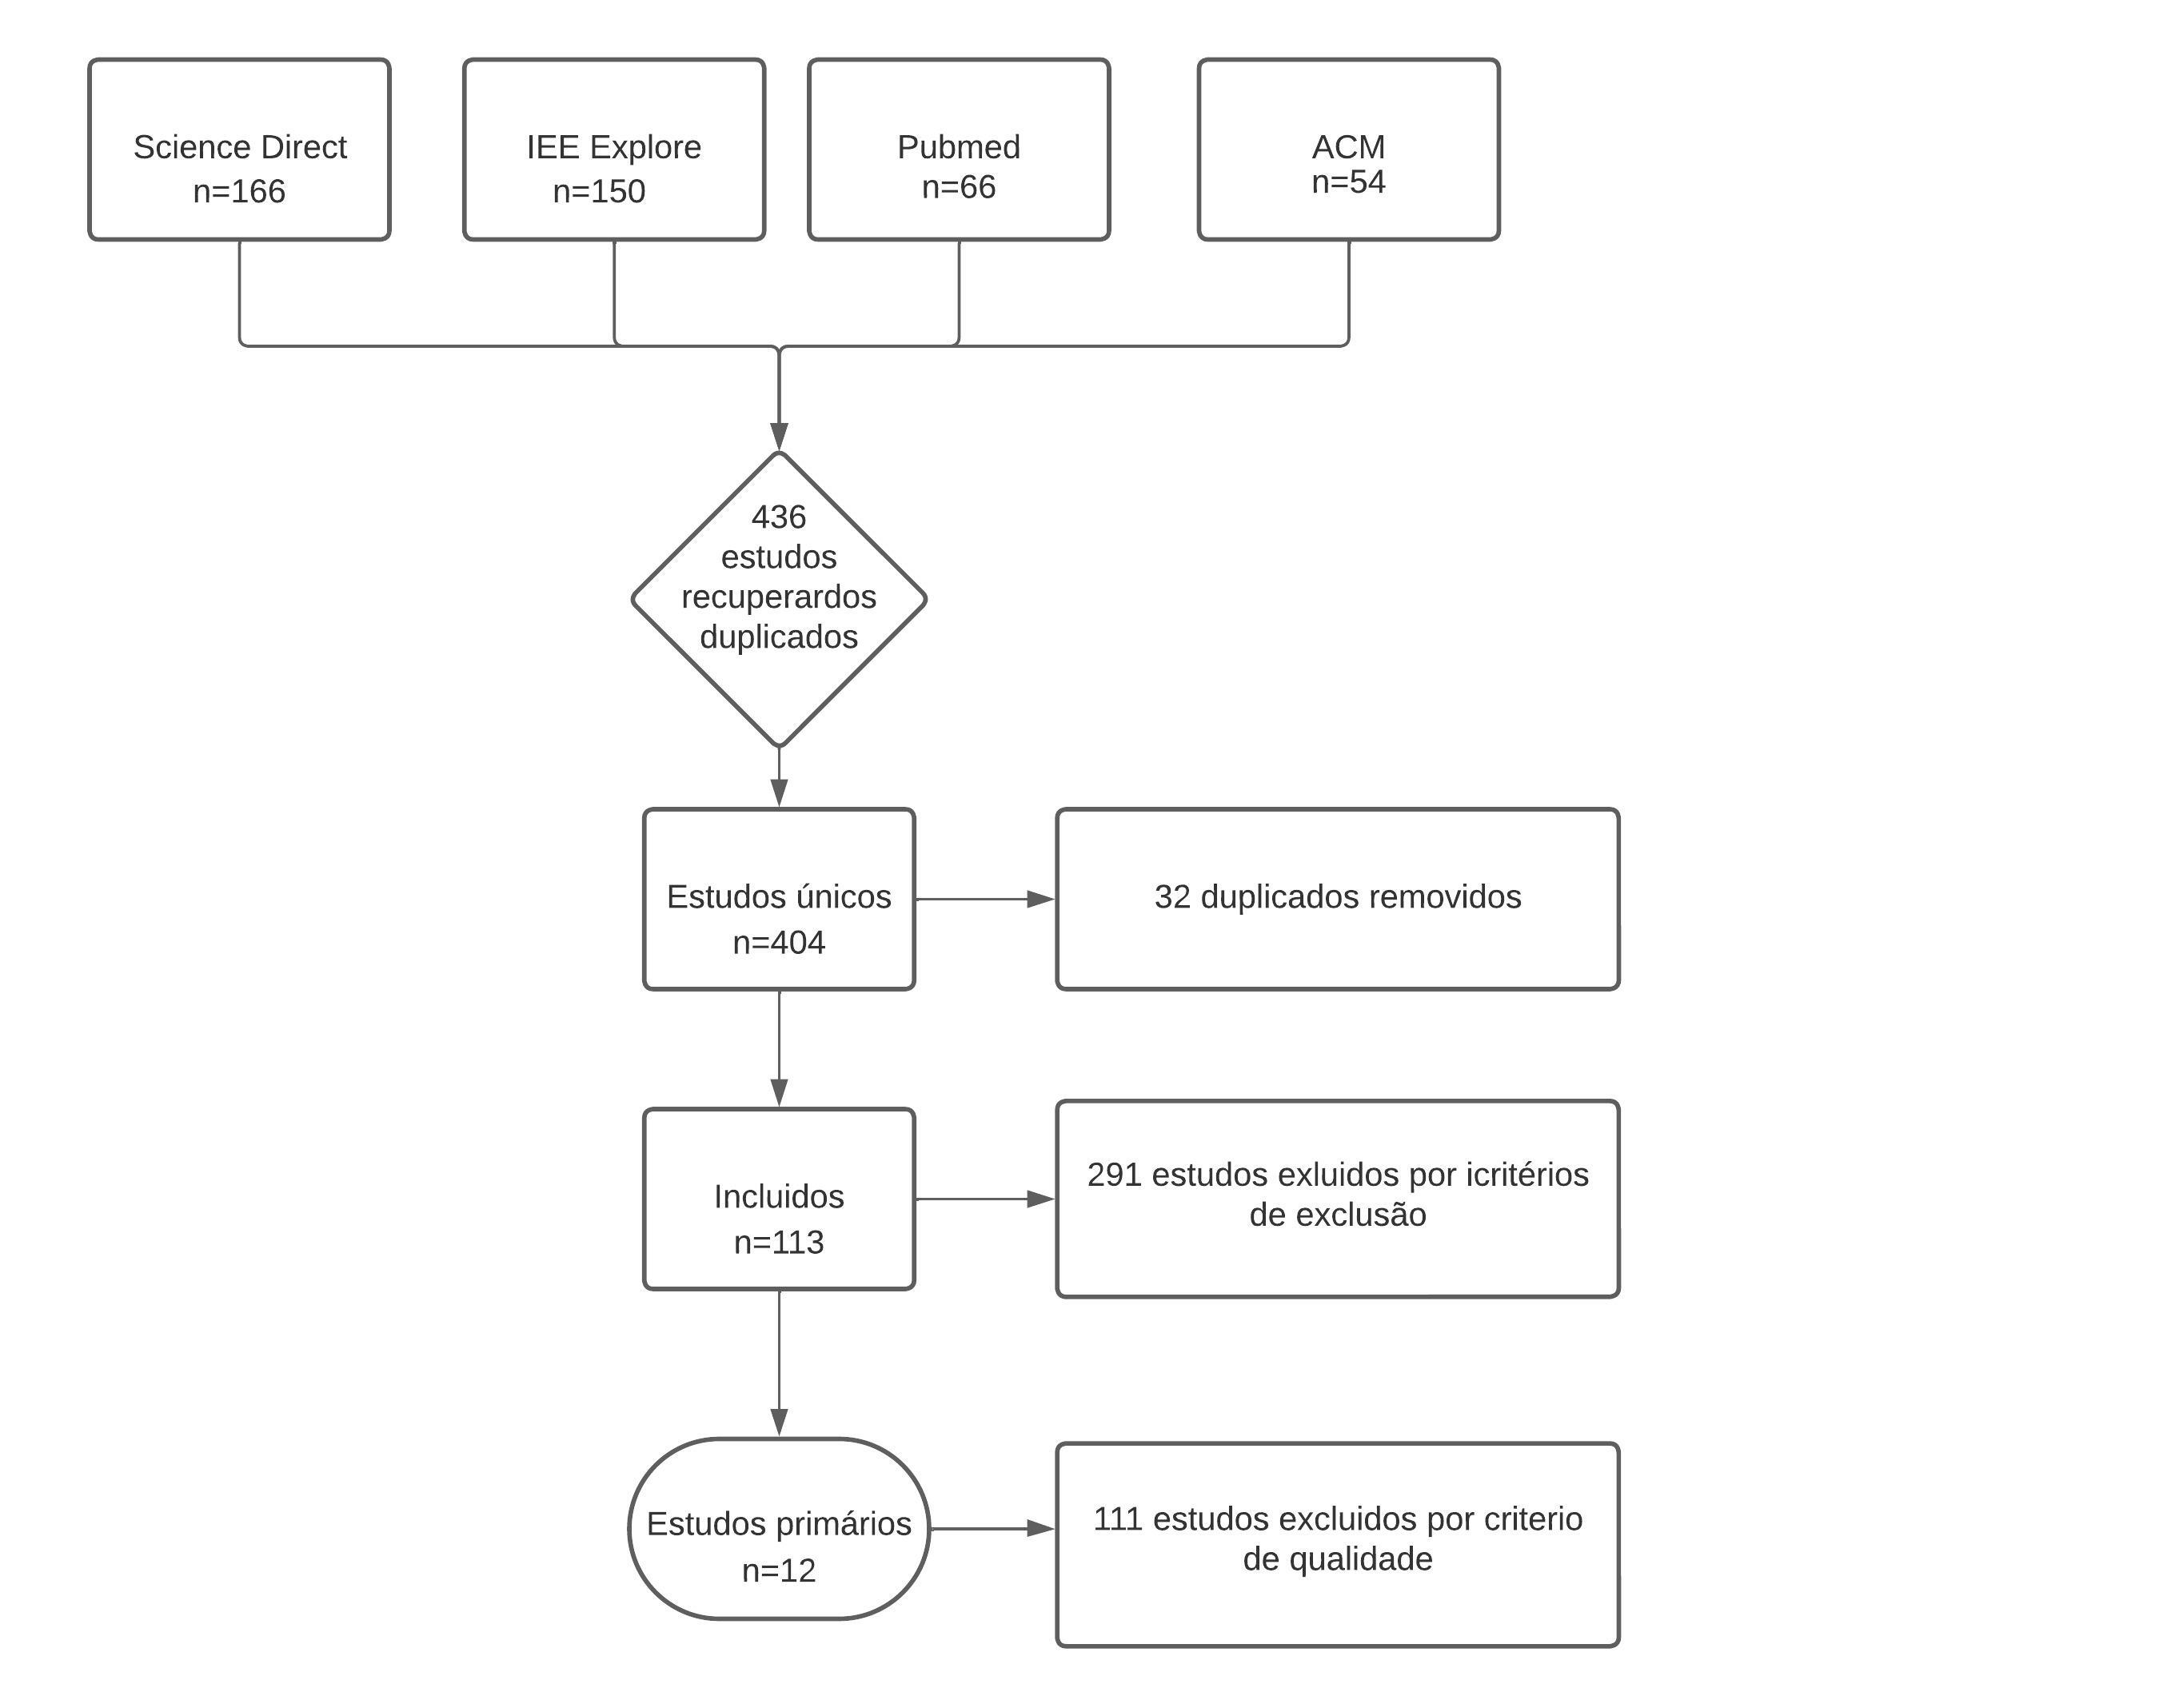
\includegraphics[width=0.8\linewidth]{capitulos/figuras/diagrama_slr.jpeg}
   \caption{Etapas da revisão sistemática da literatura.}
   \label{fig:fluxoslr}
\end{figure}

\begin{table}[!ht]
\begin{center}
\caption{Tabela de artigos selecionados}
\label{tab:trabalhos}
\resizebox{\textwidth}{!}{
\begin{tabular}{c c}
\hline
\textbf{Artigo} & \textbf{Algoritmo} \\
\hline
% 1 trabalho
\textcite{LIU2021101873} & Rede Neural Convolucional (CNN) com uma rede de atenção local \\
% 2 trabalho
\textcite{9648607} & Rede Neural Convolucional (CNN) e Rede neural Bayesiana \\
% 3 trabalho
\textcite{9335592} & Rede Neural Convolucional (CNN) \\
% 4 trabalho
\textcite{10.1001/jamacardio.2021.6059} & Rede Neural Convolucional (CNN) \\
% 5 trabalho
\textcite{Ouyang2020} & Rede Neural Convolucional (CNN) \\
% 6 trabalho
\textcite{Sun2021} & Rede Neural Convolucional (CNN) \\
% 7 trabalho
\textcite{corinzia2020neural} & Filtragem Colaborativa Neural \\
% 8 trabalho
\textcite{DONG2020101638} & AtlasNet \\
% 9 trabalho
\textcite{8931542} & Rede Neural Convolucional (CNN) \\
% 10 trabalho
\textcite{8649738} & Rede Neural Convolucional (CNN) com Arquitetura Encoder-Decoder \\
% 11 trabalho
\textcite{8586941} & DenseNet, ResNet e LSTM Bidirecional \\
% 12 trabalho
\textcite{Reynald} & Rede neural transformes e ResnetAE Encoder-Decoder\\
\hline
\end{tabular}}
\end{center}
\end{table}

\section{Estudos selecionados}
\label{Estudos selecionados}

Nesta Seção, a Seção \ref{subsec:Redes neurais convolucionais} será dedicada a uma análise detalhada dos conceitos fundamentais das redes neurais artificiais convolucionais, com um enfoque especial em sua aplicação na análise de imagens de ecocardiogramas. Esta Seção explorará a estrutura, as funcionalidades e as implicações práticas das redes convolucionais, fornecendo um entendimento aprofundado de como essas redes processam e interpretam imagens. Além disso, será apresentada uma revisão de trabalhos significativos que empregam a CNN na análise de ecocardiogramas, destacando avanços recentes e como esses estudos contribuem para o campo da imagem médica. Após delinear esses aspectos e trabalhos relacionados, a discussão evoluirá para a próxima subSeção  \ref{subsec:Redes neurais transformers}, na qual serão introduzidos os conceitos de redes transformadoras e trabalhos relacionados, abrindo um novo horizonte no contexto do processamento avançado de imagens médicas. 

\section{Redes neurais convolucionais}
\label{subsec:Redes neurais convolucionais}

%!explicação Redes neurais convolucionais


O primeiro grupo de arquitetura nos trabalhos selecionados são as redes neurais convolucionais. \textcite{CHAI2021100134} define a CNN como uma estrutura composta por camadas convolucionais, de pooling e totalmente conectadas. As camadas convolucionais se destacam por utilizar vários núcleos para processar a imagem inteira e os mapas de características intermediários, resultando na formação de diversos mapas de características.

Em um modelo de CNN, a entrada X de cada camada é estruturada em três dimensões: altura (a), largura (l) e profundidade (p), sendo que a altura é igual à largura. A profundidade, que também pode ser descrita como o número de canais, varia conforme o tipo de imagem; por exemplo, tem valor três em imagens RGB. Além disso, em cada camada convolucional, estão presentes vários núcleos ou filtros, identificados pela letra k, que também são tridimensionais, seguindo as mesmas dimensões de altura, largura e profundidade.

\textcite{Alzubaidi2021} explica as várias etapas e componentes da arquitetura de uma CNN. A camada convolucional, sendo o componente mais significativo da arquitetura, consiste em uma coleção de filtros convolucionais. Esses filtros são usados para convolucionar a imagem de entrada, que é expressa em métricas N-dimensionais, resultando na geração do mapa de características de saída. O \textit{kernel}, que se configura como uma matriz composta por uma série de valores numéricos discretos, conhecidos como pesos do \textit{kernel}, é inicialmente atribuído de forma aleatória. Existem diversas técnicas para essa inicialização, cada uma com características específicas. Conforme o treinamento avança, passando por várias \textit{epochs}, ocorre um processo de ajuste e refinamento desses pesos. Essa etapa é crucial, pois permite que o \textit{kernel} aprimore sua capacidade de identificar e extrair características relevantes dos dados de entrada, contribuindo significativamente para o processo de aprendizado da rede.

Na arquitetura de uma CNN, a operação convolucional é um processo central que difere das redes neurais tradicionais em sua abordagem de entrada de dados. Enquanto as redes neurais convencionais utilizam um formato vetorial para a entrada, as CNNs processam imagens multicanais, como as de canal único em escala de cinza ou as RGB de três canais. Para ilustrar essa operação, consideremos uma imagem em escala de cinza de 4 × 4 e um \textit{kernel} de 2 × 2 com pesos inicializados aleatoriamente. Durante a convolução, o \textit{kernel} desliza sobre a imagem, tanto horizontal quanto verticalmente, e em cada posição, o produto escalar entre a imagem e o \textit{kernel} é calculado. Esse cálculo envolve multiplicar e somar os valores correspondentes para gerar um valor escalar único, que compõe o mapa de características de saída. Este processo continua até que o \textit{kernel} não possa mais deslizar sobre a imagem.

Dois conceitos importantes na operação convolucional são o \textit{padding} e o \textit{stride}. O \textit{padding} refere-se à adição de pixels extras ao redor da borda da imagem de entrada, permitindo que o \textit{kernel} processe completamente todas as áreas da imagem, incluindo as bordas, evitando a perda de informações de borda. Isso é especialmente importante para manter o tamanho da imagem de entrada após a convolução. Por outro lado, o \textit{stride} define o tamanho do passo que o \textit{kernel} dá ao deslizar sobre a imagem. Um \textit{stride} de um, por exemplo, significa que o \textit{kernel} se move um pixel de cada vez, enquanto um \textit{stride} maior resulta em um salto de mais pixels e, consequentemente, um mapa de características com dimensões menores. A escolha do \textit{stride} e a aplicação de \textit{padding} são decisões estratégicas no design da CNN, pois influenciam diretamente na captura de características e no tamanho do mapa de características.

A camada de \textit{pooling} desempenha a função crucial de subamostrar os mapas de características que são gerados após as operações convolucionais. Este processo consiste em reduzir o tamanho dos mapas de características, criando versões menores, mas ainda preservando a maioria das informações dominantes. Antes de iniciar a operação de \textit{pooling}, tanto o \textit{stride} quanto o tamanho do \textit{kernel} são definidos. Existem vários métodos de \textit{pooling}, incluindo \textit{pooling} máximo, mínimo, médio, \textit{tree pooling}, \textit{gated pooling}, \textit{global average pooling} (GAP) e \textit{global max pooling}, sendo os métodos de \textit{pooling} máximo, mínimo e GAP os mais comuns. Apesar de sua importância na redução de dimensionalidade e na manutenção de características relevantes, a camada de \textit{pooling} pode às vezes diminuir o desempenho geral da CNN, pois, enquanto ajuda a determinar a presença de características específicas, pode não capturar sua localização exata, o que pode levar à perda de informações críticas para o modelo.

Em todas as redes neurais, inclusive as redes transformes que serão explicadas posteriormente, a função de ativação desempenha um papel fundamental, sendo responsável por transformar os dados de entrada em saída. Esta transformação envolve o cálculo de uma soma ponderada dos inputs de cada neurônio, adicionando-se o viés quando este é parte da estrutura do neurônio. A função de ativação determina a ativação ou não de um neurônio com base nesses valores de entrada, produzindo assim a saída correspondente. Em uma arquitetura de CNN, as camadas de ativação não-lineares são utilizadas após todas as camadas com pesos, conhecidas como camadas aprendíveis, que incluem as camadas totalmente conectadas (FC) e as camadas convolucionais. A natureza não-linear dessas camadas de ativação implica que o mapeamento de entrada para saída também será não-linear, permitindo que a CNN aprenda padrões mais complexos. Além disso, é crucial que a função de ativação possa ser diferenciada, uma característica extremamente importante para permitir que o erro de retro propagação seja utilizado no treinamento da rede.

\textcite{Alzubaidi2021} apresenta que diversas funções de ativação são empregadas nas CNNs, cada uma com características e equações matemáticas específicas. Entre elas estão a função Sigmoide, a função Tanh, a função ReLU e a função Leaky ReLU. A função Sigmoide aceita números reais como entrada e restringe a saída a valores entre zero e um. Sua curva é em forma de S e é matematicamente representada pela Equação \ref{eq:1}.

\begin{equation}
f(x)_{\text{sigm}} = \frac{1}{1 + e^{-x}}
\label{eq:1}
\end{equation}

A função Tanh, semelhante à Sigmoide em termos de aceitar números reais, limita a saída a valores entre -1 e 1, representada pela Equação \ref{eq:2}.

\begin{equation}
f(x)_{\text{tanh}} = \frac{e^x - e^{-x}}{e^x + e^{-x}}
\label{eq:2}
\end{equation}

A função ReLU, comumente utilizada no contexto das CNNs, transforma todos os valores de entrada em números positivos, sendo preferida devido à menor carga computacional. Sua representação matemática é definida pela Equação \ref{eq:3}.

\begin{equation}
\text{ReLU}(x) = \max(0, x)
\label{eq:3
}
\end{equation}

Uma variação da ReLU, conhecida como Leaky ReLU, foi desenvolvida para superar o problema do Dying ReLU. Diferentemente da ReLU tradicional, que anula todas as entradas negativas, a Leaky ReLU permite um pequeno valor de saída para essas entradas, evitando assim que os neurônios se tornem completamente inativos. Isso é alcançado ao multiplicar as entradas negativas por um coeficiente pequeno, garantindo a ativação contínua dos neurônios durante o treinamento. Sua representação matemática é definida pela Equação \ref{eq:4
}.

\begin{equation}
\text{Leaky ReLU}(x) = \begin{cases}
x & \text{se } x > 0, \
\alpha x & \text{se } x \leq 0
\end{cases}
\label{eq:4
}
\end{equation}

Na arquitetura de uma Rede Neural Convolucional (CNN), é comum encontrar a camada Fully Connected (FC) posicionada ao final. Esta camada caracteriza-se pela conexão de cada um de seus neurônios com todos os neurônios da camada anterior, seguindo a abordagem conhecida como totalmente conectada. Sua principal função é atuar como classificador dentro da CNN, adotando uma metodologia similar à encontrada em redes neurais perceptron multicamadas convencionais, que são um tipo de rede neural artificial feed-forward. Os dados de entrada para a camada FC provêm da última camada de pooling ou convolucional. Esses dados são transformados em um vetor, que é formado a partir do achatamento dos mapas de características.

Por fim, \textcite{Alzubaidi2021} descreve que as funções de perda na arquitetura de CNNs são componentes fundamentais, aplicadas na camada de saída, que é a última etapa da estrutura da rede. Essas funções desempenham o papel vital de calcular o erro de predição durante o treinamento do modelo, avaliando a diferença entre os resultados reais e os previstos pela CNN. O processo de aprendizado da rede é fortemente influenciado pela otimização desse erro, pois orienta a CNN na correção e aprimoramento de suas previsões. Para realizar o cálculo do erro, as funções de perda utilizam dois parâmetros chave: o output estimado pela CNN, conhecido como previsão, e o output real, referido como rótulo. Dependendo da natureza do problema abordado, são empregadas diversas funções de perda, cada uma adaptada para tratar especificidades dos dados e do modelo em questão, sendo a escolha da função de perda apropriada um fator crítico para o sucesso do treinamento da rede.

A função de perda de Entropia Cruzada ou Softmax é comumente utilizada em problemas de classificação multiclasse, produzindo uma probabilidade de saída e frequentemente substituindo a função de erro quadrático definido pela Equação \ref{eq:entro}.

\begin{equation}
\text{Softmax} = -\sum_{c=1}^{M} y_{o,c} \log(p_{o,c})
\label{eq:entro}
\end{equation}

Outra função importante é a função de perda Euclidiana, amplamente usada em problemas de regressão e também conhecida como erro quadrático médio pela Equação \ref{eq:eucl}.

\begin{equation}
\text{Euclidean Loss} = \frac{1}{2N} \sum_{i=1}^{N} (y_i - \hat{y}_i)^2
\label{eq:eucl}
\end{equation}

A Função de Perda Hinge é comum em problemas de classificação binária e é especialmente importante para Máquinas de Vetores de Suporte (SVMs), onde busca maximizar a margem em torno de classes objetivas duais e é definido pela Equação \ref{eq:hing
}.

\begin{equation}
\text{Hinge Loss} = \sum_{i=1}^{N} \max(0, 1 - y_i \cdot \hat{y}_i)
\label{eq:hing
}
\end{equation}

Após o desempenho da AlexNet na competição ImageNet, as Redes Neurais Convolucionais consolidaram-se como a metodologia predominante no aprendizado profundo para aplicações em visão computacional, conforme destacado por \textcite{CHAI2021100134}. Desenvolvida por \textcite{NIPS2012_c399862d}, a AlexNet distinguiu-se como a primeira rede neural a obter êxito no ImageNet Large Scale Visual Recognition Challenge, um concurso internacional de grande prestígio na área de reconhecimento de imagens. Este marco na evolução das CNNs demonstrou de maneira inequívoca a capacidade destas redes de superarem as abordagens tradicionais no campo do reconhecimento de imagens. A arquitetura da AlexNet, compreendendo oito camadas, incluindo cinco camadas convolucionais e três totalmente conectadas, foi treinada em um vasto conjunto de dados do ImageNet, que abrange mais de 1,2 milhões de imagens em 1.000 categorias. Este treinamento resultou em uma taxa de erro de apenas 16,4\% no desafio.

Após os avanços da AlexNet no campo das CNNs para visão computacional, \textcite{https://doi.org/10.48550/arxiv.1409.1556} ampliou as fronteiras do conhecimento estabelecidas pela AlexNet, explorando o efeito da profundidade aumentada em redes convolucionais para o reconhecimento de imagens em larga escala. Ao focar em arquiteturas com até 19 camadas convolucionais, eles demonstraram que um aumento na profundidade da rede poderia resultar em uma melhoria notável na precisão da classificação de imagens. 


\textcite{he2015deep} apresentaram um novo design de redes neurais convolucionais com a introdução da ResNet, uma rede de arquitetura residual. Eles argumentaram que aprender uma função residual em relação à entrada de uma camada é mais eficiente do que aprender os parâmetros da camada independentemente das entradas. A ResNet, com suas 152 camadas, demonstrou ser significativamente mais profunda do que as VGG Nets, sendo oito vezes mais profunda. A chave para o sucesso dessa rede estava na utilização de várias camadas de parâmetros para aprender a representação dos resíduos entre a entrada e a saída, em vez de aprender diretamente o mapeamento entre entrada e saída como em redes CNN convencionais (por exemplo, AlexNet, VGG).

As VGG Nets, introduzidas por \textcite{simonyan2015deep}, são redes neurais convolucionais projetadas para aumentar a profundidade da rede utilizando pequenas convoluções de 3x3 pixels, empilhadas uma sobre a outra. Este design simples, mas eficaz, permitiu que a rede fosse treinada de forma mais eficiente e com melhor desempenho em tarefas de classificação de imagens, especialmente no ImageNet Large Scale Visual Recognition Challenge (ILSVRC).

Com o aumento das conexões diretas, a ResNet não apenas promoveu uma solução para o problema do gradiente desvanecente, mas também fortaleceu a propagação das características, incentivou a reutilização de características e reduziu substancialmente o número de parâmetros necessários. A VGG, por sua vez, focou em uma estrutura mais simples e uniforme, porém com um aumento significativo na profundidade em comparação com redes anteriores, permitindo uma maior capacidade de aprendizado e uma melhor generalização.


Proposto por \textcite{https://doi.org/10.48550/arxiv.1709.02371} a PWC-Net (Pyramid, Warping, and Cost Volume Network), é uma  arquitetura de rede neural convolucional desenvolvida para estimar o fluxo óptico em imagens, uma técnica crucial em várias aplicações de visão computacional. O fluxo óptico é o padrão de movimento aparente de objetos e superfícies em uma cena visual, resultante do movimento relativo entre um observador e a cena. Esta rede é especialmente útil em tarefas como rastreamento de objetos, reconhecimento de ações e navegação autônoma.A PWC-Net se destaca por sua abordagem de três etapas para processar imagens e estimar o movimento. Primeiramente, cria-se uma pirâmide de características para cada imagem de entrada. Esta pirâmide consiste em múltiplas versões reduzidas da imagem original, cada uma oferecendo um nível diferente de detalhes. Ao extrair características em várias escalas, a rede consegue identificar padrões de movimento tanto em nível macro quanto micro, ajudando a entender o movimento global e detalhes finos dentro da cena.

Os parágrafos anteriores descreveram as CNNs. Nos próximos parágrafos, serão listadas algumas aplicações práticas das CNNs, conforme indicado nos estudos da revisão sistemática.

% 1 trabalho
\textcite{LIU2021101873} introduz a Deep Pyramid Local Attention Network (DPLAN), uma arquitetura de rede neural profunda desenvolvida para a segmentação de estruturas cardíacas em ecocardiografia bidimensional (2D). A DPLAN combina uma rede de detecção de características baseada na arquitetura ResNet com uma rede de atenção local, utilizando o conceito de atenção para focalizar áreas específicas da imagem, melhorando a precisão e robustez da segmentação. Essa integração permite à rede aprender representações robustas mesmo em imagens com alta variabilidade, enquanto um esquema de treinamento multi-escala habilita a identificação de características em diferentes escalas, importante para a segmentação de estruturas cardíacas complexas. Na avaliação com um conjunto de dados composto por ecocardiogramas 2D de 100 pacientes, a DPLAN demonstrou uma notável precisão de segmentação, atingindo 92,5\% para o ventrículo esquerdo, 91,2\% para o ventrículo direito e 88,0\% para a parede livre do ventrículo esquerdo. Esses resultados superam os obtidos por métodos alternativos de segmentação, solidificando a eficácia  da abordagem proposta e indicando seu potencial para aprimorar diagnósticos e tratamentos de doenças cardíacas. Além das contribuições mencionadas, a DPLAN destaca-se por sua simplicidade e facilidade de implementação, tornando-a uma ferramenta eficiente em termos de computação. Essas características adicionais reforçam a posição promissora da DPLAN como uma solução viável e eficaz para a segmentação de estruturas cardíacas em ecocardiografia 2D .

% 2 trabalho

\textcite{9648607} apresenta que entro do contexto de imagens cardíacas, a segmentação de ecocardiogramas emerge como uma peça fundamental no diagnóstico cardíaco, proporcionando a avaliação  da função ventricular esquerda. Contudo, as estratégias de aprendizado profundo voltadas para essa tarefa enfrentam desafios substanciais, notadamente a aquisição de dados de treinamento em quantidade suficiente e o desenvolvimento demorado de modelos de alta qualidade . Os próximos parágrafos descrevem  as abordagens e resultados apresentados.

Para abordar esses desafios, um pipeline de aprendizado de máquina totalmente automatizado foi proposto, empregando técnicas de aprendizado ativo e busca por arquiteturas neurais (NAS). O aprendizado ativo desempenha um papel fundamental, selecionando inteligentemente os pontos de dados mais informativos de um conjunto de dados maior para rotulação por especialistas. Esta abordagem é particularmente benéfica no domínio da imagem médica, onde a rotulação manual de dados pode ser extremamente demorada e requer conhecimento especializado. Ao focar nas imagens de ecocardiograma mais valiosas que contribuirão mais para o processo de aprendizagem, o aprendizado ativo reduz significativamente o volume de dados que precisam ser anotados manualmente. Isso não apenas economiza tempo e recursos, mas também garante que o processo de aprendizagem esteja focado nos dados mais críticos.

O pipeline também emprega a NAS, especificamente uma Pesquisa de Arquitetura Neural de Codificador-Decodificador (EDNAS) projetada para tarefas de segmentação de imagens. A NAS automatiza o processo de projetar arquiteturas de redes neurais, que tradicionalmente é uma tarefa manual e complexa. O sistema EDNAS testa e otimiza iterativamente várias configurações de redes neurais para descobrir a arquitetura mais eficiente e eficaz para a tarefa específica de segmentação de ecocardiogramas. Esta abordagem automatizada acelera o desenvolvimento de modelos de aprendizado profundo altamente precisos e personalizados sem exigir intervenção manual extensa.

Ao combinar essas duas técnicas, o pipeline alcança uma abordagem mais eficiente e escalável para análise de imagens médicas. O aprendizado ativo garante que os dados de treinamento sejam da mais alta relevância e qualidade, enquanto a NAS otimiza a arquitetura da rede neural para um desempenho superior. Essa integração leva a uma redução significativa no trabalho manual envolvido na rotulação de dados e no desenvolvimento de modelos, mantendo alta precisão nas tarefas de segmentação.

O pipeline foi testado em um conjunto de dados de referência de imagens de ecocardiograma, demonstrando que atinge uma precisão de segmentação comparável a abordagens tradicionais de aprendizado profundo, enquanto utiliza apenas dois quintos do conjunto de dados de treinamento. Essa notável redução nos requisitos de dados destaca a eficácia do pipeline proposto em aliviar a carga de rotulagem e acelerar o desenvolvimento de modelos de aprendizado profundo para a segmentação de ecocardiogramas.

Os resultados obtidos revelam que o pipeline alcançou uma precisão de segmentação de 92,7\%, evidenciando sua capacidade de competir com abordagens convencionais que demandam um conjunto de dados completo de treinamento. Além disso, esse desempenho foi atingido com apenas 400 imagens de treinamento, representando uma significativa economia de dados. Essa redução substancial nos requisitos de dados sublinha a eficácia do pipeline em simplificar o processo de rotulagem e impulsionar o desenvolvimento de modelos de aprendizado profundo destinados à segmentação de ecocardiogramas.


% 3 trabalho

O estudo \textcite{9335592} introduz um framework baseado em aprendizado profundo para estimativa de movimento em ecocardiografia, com foco na automatização da análise da função miocárdica. Utilizando a arquitetura PWC-Net na construção do estimador de movimento, o estudo reflete um aproveitamento das capacidades avançadas dessa arquitetura em tarefas de estimativa de movimento, adaptando-a especificamente para as necessidades da ecocardiografia. O modelo desenvolvido demonstra uma alta precisão, com um erro médio de ponto final de apenas (0,06 ± 0,04) mm por quadro em dados simulados. O modelo também demonstra adaptabilidade a artefatos de imagem, especialmente em situações de perda de sinal, um desafio comum na ecocardiografia devido a fatores como atenuação de sinal e movimentos rápidos do coração. Essa capacidade de adaptação é possibilitada por treinamento com aumentos de imagem pertinentes, o que permite ao sistema manter sua precisão mesmo em condições variáveis encontradas em imagens ecocardiográficas reais. Nos próximos parágrafos, serão detalhadas as abordagens e resultados deste estudo.

A arquitetura PWC-Net não apresenta apenas uma estimativa de movimento, mas também um pipeline abrangente para análise automatizada de imagens miocárdicas funcionais. Em sua fase inicial, o sistema integra uma rede interna de classificação de visão cardíaca (CVC), desenvolvida para assegurar a precisão das janelas acústicas. Esta rede é treinada e avaliada em extensos conjuntos de dados, projetada para identificar até oito distintas incidências cardíacas cruciais para o estudo. A arquitetura da rede é complexa e bem elaborada, composta por diversos níveis que incorporam blocos de filtros de convolução, normalização em lote, ativação PReLU e pooling máximo. A entrada da rede consiste em imagens de ultrassom padrão convertidas em modo B, enquanto a saída gera uma pontuação de confiança para cada classe detectada. Este sistema demonstra uma eficiência notável, alcançando uma precisão  de 98\%, evidenciando sua capacidade em prover análises confiáveis e precisas no contexto da imagem cardíaca.

Paralelamente, a detecção de fases cardíacas é realizada por meio de uma rede convolucional, capaz de classificar diástole e sístole diretamente das imagens em modo B. Esta rede inclui várias camadas de convoluções 3D, normalização em lote, ativação ReLU, pool máximo e módulos de memória de curto prazo longo (LSTM). Ela foi treinada e validada em um conjunto de dados extenso e demonstrou uma precisão significativa na identificação das fases cardíacas, contribuindo para a precisão geral do sistema.

Após a classificação e detecção de fases, o pipeline envolve a segmentação miocárdica usando uma rede de segmentação baseada em uma adaptação da arquitetura U-Net. Esta rede é capaz de classificar distintas partes da imagem cardíaca, sendo essencial para a identificação e análise do miocárdio. Foi treinada com imagens de incidências específicas e demonstrou eficácia e eficiência, com um tempo de execução impressionantemente rápido em uma GPU.

A etapa seguinte envolve a extração da linha central do miocárdio, definida pelo contorno da segmentação miocárdica e a localização das bordas endo- e epicárdicas. Essa linha central é crucial para as etapas subsequentes de análise e medição. No que diz respeito à estimativa de movimento, o pipeline oferece flexibilidade, permitindo o uso de diferentes métodos. Neste estudo, foram empregadas quatro variantes, incluindo um método tradicional de fluxo óptico e versões adaptadas da rede PWC-Net. Esses métodos geram um mapa de deslocamento denso, crucial para a análise detalhada do movimento miocárdico.

A atualização de rastreamento no sistema proposto é efetuada pela propagação dos pontos da linha central utilizando o campo de deslocamento, oferecendo uma abordagem alternativa que permite a utilização direta da segmentação, sem a necessidade de recorrer ao método de estimativa de movimento. Esta etapa do processo é caracterizada por sua flexibilidade, podendo incorporar técnicas adicionais de estimação de estados, ainda que não tenham sido profundamente exploradas neste estudo. Em seguida, as medidas clínicas são extraídas a partir desta linha central, incluindo a avaliação da cepa Lagrangiana e a análise da deformação. Essas medidas são calculadas com base no comprimento de referência, proporcionando insights valiosos sobre a condição e o funcionamento do miocárdio, elementos essenciais para a compreensão detalhada da saúde cardíaca.

% 4 trabalho

 No contexto da análise cardíaca via ecocardiografia, o artigo de \textcite{10.1001/jamacardio.2021.6059} aborda a avaliação da hipertrofia ventricular esquerda (HVE) utilizando técnicas de aprendizado profundo. A HVE é caracterizada pelo espessamento das paredes do ventrículo esquerdo e é um indicador importante para o risco de insuficiência cardíaca e outros eventos cardiovasculares. A detecção e caracterização precoce da HVE são essenciais para o manejo eficaz do paciente. Neste contexto, o estudo apresenta o EchoNet-LVH, um algoritmo de aprendizado profundo desenvolvido para medir a espessura da parede do ventrículo esquerdo e identificar pacientes com HVE a partir de imagens de ecocardiografia. O algoritmo foi treinado em um conjunto de dados abrangente, incluindo ecocardiogramas de pacientes com e sem HVE, e alcançou uma precisão de 95\% na identificação de pacientes com HVE, superando os métodos convencionais que são frequentemente subjetivos e sujeitos à variabilidade interobservador.

A arquitetura do EchoNet-LVH se baseia em uma rede neural convolucional (CNN) 3D, projetada para processar e analisar dados volumétricos, como imagens 3D. Esta arquitetura inclui várias camadas: uma camada de entrada, que recebe a imagem de ecocardiografia, camadas convolucionais, que extraem características da imagem; camadas de pooling, que reduzem a dimensão dos recursos extraídos; camadas de upsampling, que aumentam a dimensão desses recursos; e uma camada de saída, que produz a medição da espessura da parede do ventrículo esquerdo. O treinamento do EchoNet-LVH foi focado no ajuste dos parâmetros da CNN 3D para que o algoritmo pudesse aprender a associar imagens de ecocardiografia com medições precisas da espessura da parede do ventrículo esquerdo.

Em termos de aplicação clínica, o EchoNet-LVH oferece vantagens como automação completa, que economiza tempo e melhora a consistência nas avaliações, e objetividade, que pode reduzir a variabilidade interobservador. O algoritmo também fornece informações detalhadas sobre a espessura da parede do ventrículo esquerdo, importantes para a caracterização da gravidade da HVE. Portanto, o desenvolvimento do EchoNet-LVH contribui para o avanço na avaliação da HVE, potencialmente melhorando a precisão e eficiência do diagnóstico e manejo dessa condição, o que pode resultar em melhores desfechos clínicos para os pacientes.

% 6 trabalho

Ainda seguindo no grupo de pesquisa do artigo anterior \textcite{Ouyang2020} apresenta uma abordagem utilizando a aprendizagem profunda para a avaliação contínua da função cardíaca a partir de vídeos de ecocardiografia. Esta técnica é importante para o diagnóstico e tratamento de diversas condições cardíacas, incluindo insuficiência cardíaca, doença arterial coronariana e arritmias. O trabalho introduz o EchoNet-Dynamic, um modelo de aprendizado profundo, especialmente desenvolvido para medir a fração de ejeção do ventrículo esquerdo (FEVE) e identificar pacientes com insuficiência cardíaca. 

O modelo utiliza uma Rede Neural Convolucional (CNN) que incorpora convoluções atrous, uma técnica  que permite a captura de padrões em diferentes escalas. As convoluções atrous são eficazes em lidar com espaçamentos irregulares nos dados, um desafio comum nas imagens de ecocardiografia. Essa abordagem  é crucial para analisar com precisão os complexos padrões encontrados nos dados de ecocardiografia. Ao contrário das convoluções tradicionais, que processam dados com espaçamentos regulares, as convoluções atrous adaptam-se melhor aos dados irregulares, aumentando a eficácia do modelo na identificação de características importantes para o diagnóstico e análise cardíaca.

Além das convoluções atrous, o EchoNet-Dynamic também emprega convoluções espaciotemporais. Essa integração de informações espaciais e temporais é uma inovação significativa no campo do processamento de dados médicos, especialmente para imagens de vídeo, onde tanto a dimensão espacial quanto a temporal são fundamentais para uma análise completa. A estrutura do modelo é projetada para otimizar a extração e o processamento de informações. Inicia-se com camadas de entrada que recebem os vídeos de ecocardiografia, seguidas por camadas convolucionais para extração de recursos. Estas são acompanhadas de camadas de pooling, que reduzem a dimensão dos dados, e camadas de upsampling, que ampliam os recursos extraídos. Por fim, o modelo conclui com uma camada de saída que fornece estimativas precisas da fração de ejeção do ventrículo esquerdo ou classificações de insuficiência cardíaca.

O desempenho do EchoNet-Dynamic foi avaliado em um conjunto de dados de 10030 pacientes, demonstrando uma eficácia notável, com 97\% de precisão na identificação de pacientes com insuficiência cardíaca. Esta taxa de sucesso supera significativamente os métodos tradicionais de avaliação da FEVE. O estudo de \textcite{Ouyang2020}. marca um avanço significativo na avaliação da função cardíaca, apresentando o EchoNet-Dynamic como uma ferramenta precisa e não invasiva para identificar pacientes com insuficiência cardíaca, potencializando o diagnóstico e tratamento de várias condições cardíacas. Apesar dos resultados promissores, o estudo possui limitações, incluindo o tamanho relativamente pequeno da amostra e a falta de representatividade da população geral. Além disso, a validação do EchoNet-Dynamic ocorreu em um único centro, o que pode restringir a generalização dos resultados. 

% 7 trabalho

\textcite{Sun2021} propõe um método baseado em inteligência artificial, especificamente uma rede neural convolucional (CNN), para triagem de disfunção do ventrículo esquerdo em pacientes, utilizando como única fonte de dados os eletrocardiogramas (ECG) padrão de 12 derivações. A CNN é uma classe de redes neurais profundas reconhecida por sua eficácia no reconhecimento de imagens médicas, adaptada aqui para a análise de dados de ECG. Nos parágrafos seguintes, serão detalhadas as abordagens e resultados desse estudo.

Para o desenvolvimento do modelo, dados de ECG e ecocardiograma transtorácico (TTE) foram coletados, incluindo valores da fração de ejeção do ventrículo esquerdo (FEVE). Esses dados foram pareados por paciente, e, no caso de múltiplas medições para um mesmo paciente, apenas o par de dados mais antigo foi considerado para análise. Os pares ECG-TTE foram randomicamente distribuídos em conjuntos de treinamento, validação e teste, para desenvolver e avaliar o modelo de CNN. Os indicadores de desempenho do modelo incluíram acurácia geral, sensibilidade, especificidade, valor preditivo positivo e negativo.

No total, foram analisados retrospectivamente 26.786 pares de eletrocardiogramas (ECG) e ecocardiograma transtorácico (TTE), distribuídos em 21.732 para treinamento, 2.530 para validação e 2.530 para testes. O modelo CNN resultante demonstrou uma acurácia geral de 73.9\%, sensibilidade de 69.2\%, especificidade de 70.5\%, valor preditivo positivo de 70.1\% e valor preditivo negativo de 69.9\% no conjunto de testes.


% 8 trabalho

\textcite{corinzia2020neural} apresentam uma metodologia baseada em filtragem colaborativa neural para a segmentação da válvula mitral em imagens de ecocardiografia. Este método é notável por sua capacidade de aprender a segmentar a válvula mitral de forma não supervisionada, sem a necessidade de anotações manuais. Assim como no estudo apresentados anteriormente , a aplicação de redes neurais convolucionais desempenha um papel central, mas aqui, elas são usadas para classificar pixels em imagens, determinando sua pertinência à válvula mitral. 

O método não requer anotações manuais e pode aprender a segmentar a válvula mitral a partir de um conjunto de dados não supervisionado. O método consiste em duas etapas: uma etapa de filtragem colaborativa, que aprende uma representação latente dos pixels da imagem, e uma etapa de segmentação, que usa uma rede neural convolucional para classificar os pixels como pertencentes ou não à válvula mitral. Os autores avaliam o método em um conjunto de dados de 100 imagens de ecocardiografia e mostram que ele alcança resultados comparáveis aos de métodos supervisionados, com uma precisão média de 0,86 e um coeficiente de Dice médio de 0,76. O método também é robusto a variações na qualidade da imagem, no ângulo de visão e na forma da válvula mitral.

% 9 trabalho

\textcite{DONG2020101638} descreve um método para a segmentação 3D do ventrículo esquerdo (VE) em ecocardiografia 3D (3DE). A arquitetura proposta foca no uso de uma rede denominada AtlasNet, que se baseia em um único atlas para fornecer informações sobre a estrutura anatômica do VE. A escolha de utilizar um único atlas, em vez de múltiplos, visa simplificar o processo de segmentação. Esta simplificação é alcançada ao evitar a complexidade de selecionar e combinar informações de vários atlas, uma prática comum em métodos baseados em multiatlas. Apesar dessa simplificação, a precisão da segmentação é mantida. Nos parágrafos seguintes, serão detalhadas as abordagens e resultados desse estudo.

Um atlas, no contexto da imagiologia médica, é um modelo ou mapa referencial que representa a estrutura anatômica padrão de um órgão ou região corporal. Esse modelo é usualmente construído a partir de uma série de imagens médicas de diferentes pacientes, servindo como um guia para a identificação e segmentação de estruturas anatômicas em novas imagens.

A AtlasNet integra o conhecimento prévio do atlas, permitindo representar com precisão a estrutura básica do VE em 3D. A rede aprende parâmetros de transformação específicos para a deformação do atlas, otimizando-os através de uma abordagem de retropropagação de ponta a ponta. Esses parâmetros de transformação são representados como um pequeno número de nós, tornando o sistema eficaz mesmo com uma quantidade limitada de dados anotados. Além da rede de atlas, o método incorpora uma nova restrição de consistência de informação multinível, que melhora o desempenho do modelo em ambientes anatômicos complexos. A estrutura também inclui um Couple-GAN (Generative Adversarial Networks) para modelar informações semânticas globais, proporcionando uma abordagem mais holística e integrada.

Quanto aos resultados alcançados, o método demonstrou que satisfaz o requisito de eficiência da prática clínica. Os experimentos comprovaram que o método proposto obteve melhores resultados de segmentação e maior velocidade de inferência em comparação com outros métodos. A distância média da superfície, a distância média da superfície de Hausdorff e o índice médio de dados foram 1,52 mm, 5,6 mm e 0,97, respectivamente. A superfície de Hausdorff refere-se a uma medida matemática usada para quantificar a distância entre duas superfícies. Ela representa a maior distância de um ponto de uma superfície a qualquer ponto da outra superfície, oferecendo uma maneira de avaliar a precisão na sobreposição de imagens ou segmentações. Essa medida é particularmente útil na área médica para comparar segmentações de imagens geradas por algoritmos com as realizadas por especialistas humanos. Além disso, o método é eficiente e seu tempo de inferência é de apenas 0,02 segundos.

% 10 trabalho

O artigo de \textcite{8931542} detalha um método de segmentação automática do anel mitral em ecocardiografia transesofágica tridimensional. Utilizando uma rede neural convolucional 2D profunda, o método analisa planos 2D para prever as coordenadas do anel mitral, empregando a simetria em torno da linha central do ventrículo esquerdo e aplicando regularização nas previsões de planos adjacentes para assegurar a continuidade.

Os resultados demonstram a eficácia do modelo na segmentação automática do anel mitral, apresentando um erro médio de 2,0 mm com desvio padrão de 1,9 mm, o que evidencia a precisão da técnica. Este avanço mostra a potencialidade do método em automatizar a quantificação de parâmetros do anel mitral, minimizando a necessidade de intervenção manual e reduzindo a variabilidade entre diferentes observadores.

% 11 trabalho

\textcite{8649738} apresenta uma avaliação aprofundada do potencial dos métodos de rede neural na segmentação de imagens ecocardiográficas 2D, utilizando o dataset CAMUS, que é uma base de dados especializada composta por imagens ecocardiográficas de dois e quatro compartimentos de 500 pacientes, criada pelos autores. Nos parágrafos seguintes, serão detalhadas as abordagens e resultados desse estudo.

Para testes, foram utilizadas redes com uma estrutura de encoder-decoder, uma abordagem eficaz e comprovada na área de imagens médicas. Essas redes possuem duas partes principais: o encoder, que realiza operações de convolução e redução de tamanho das imagens para extrair características importantes, e o decoder, que reconstrói uma imagem segmentada a partir dessas características, aumentando progressivamente seu tamanho. Entre as arquiteturas mais notáveis usadas está o modelo U-Net, que se destaca por suas conexões diretas entre as partes do encoder e do decoder. Essas conexões ajudam a preservar detalhes importantes que podem se perder durante a redução de tamanho no encoder, além de contribuir para a estabilidade dos gradientes no processo de aprendizado da rede.

Além do U-Net, foram testados outros modelos com base em estruturas de encoder-decoder, incluindo variações otimizadas para velocidade (U-Net 1) e precisão (U-Net 2), e o ACNN, que combina uma arquitetura de segmentação com uma perda auxiliar. Esta perda auxiliar ajuda a ajustar a saída da segmentação para se adequar a uma representação compacta e não linear da anatomia, baseada em uma rede de autoencoder. Este método ajuda a garantir que a segmentação esteja em conformidade com a estrutura anatômica esperada, aumentando a precisão.

Outro modelo testado foi o Stacked Hourglasses (SHG), que integra três redes encoder-decoder sucessivas, onde as duas primeiras funcionam como blocos residuais e a terceira produz o resultado final da segmentação. Cada uma dessas redes é acompanhada por uma perda de segmentação intermediária, uma técnica conhecida como supervisão profunda, que ajuda a guiar o treinamento da rede para uma melhor precisão. Por fim, o U-Net++, outra variação testada, também emprega a técnica de supervisão profunda, mas com camadas adicionais de convolução formando conexões densas.

Os resultados mostram que as arquiteturas baseadas em encoder-decoder superam os métodos não baseados em aprendizado profundo. Eles reproduzem com alta fidelidade a análise de especialistas para volumes ventriculares esquerdo diastólicos e sistólicos, com uma correlação média de 0,95 e um erro médio absoluto de 9,5 ml. Embora os resultados para a fração de ejeção do ventrículo esquerdo sejam mais variados, eles ainda são comparáveis aos escores inter-observadores e ligeiramente inferiores aos intra-observadores.

% 12 trabalho

\textcite{8586941} apresenta um método  para a detecção de quadros de fim de sístole (ES) e fim de diástole (ED) em ecocardiogramas. Utilizando uma combinação de Redes Neurais Convolucionais sendo elas a DenseNet, ResNet e Redes Neurais Recorrentes como memória de curto prazo longo, LSTM bidirecional.

Os resultados do estudo demonstram um desajuste médio de apenas 0,20 quadros para ED e 1,43 quadros para ES. Essa precisão está dentro da variabilidade interobservador para detecção manual, evidenciando a eficácia e aplicabilidade prática do método em um amplo conjunto de dados de ecocardiogramas, promovendo avanços significativos na análise automática de imagens cardíacas.

As abordagens mencionadas nessa Seção  destacam avanços significativos na segmentação e análise de ecocardiogramas, utilizando redes neurais convolucionais (CNNs) e técnicas de aprendizado profundo. As características comuns entre os trabalhos incluem a utilização de CNNs para extrair e analisar características relevantes das imagens cardíacas, a adaptação de arquiteturas avançadas como PWC-Net, U-Net e suas variações, e a implementação de estratégias de aprendizado ativo e NAS para otimizar o processo de treinamento e melhorar a precisão dos modelos. No entanto, os desafios persistem, como a necessidade de grandes quantidades de dados anotados para treinamento, a complexidade computacional envolvida no processamento de imagens médicas e a adaptação de modelos para lidar com variabilidades intrínsecas das imagens de ecocardiogramas, como artefatos e ruído.

Esses desafios e características comuns estabelecem a base para a transição para a próxima Seção, onde exploraremos redes transformadoras (transformers). Essas redes oferecem uma nova abordagem para o processamento avançado de imagens médicas, prometendo superar algumas das limitações das CNNs e abrir novas possibilidades para a análise de ecocardiogramas. A próxima subSeção \ref{subsec:Redes neurais transformers} apresentará os conceitos fundamentais das redes tranformers e revisará trabalhos significativos que empregam essas redes na análise de imagens médicas.


\section{Redes neurais transformers}
\label{subsec:Redes neurais transformers}

As redes neurais Transformadoras são uma arquitetura que foi proposta  por \textcite{https://doi.org/10.48550/arxiv.1706.03762}. Essas redes foram projetadas especificamente para tarefas de processamento de linguagem natural (PLN), como tradução automática, resumo de texto e geração de texto, demonstrando se extremamente eficazes nessas tarefas, superando outras arquiteturas de redes neurais em muitos casos.

Pesquisas recentes vêm demonstrando que os módulos transformadores são capazes de substituir completamente as convoluções padrão em redes neurais profundas. Essa inovação deu origem aos Transformadores de Visão (ViTs), que operam em sequências de patches de imagens. Desde sua introdução, os modelos ViT têm impulsionado o estado da arte em uma ampla gama de tarefas de visão computacional. Eles têm sido aplicados com sucesso na classificação de imagens, detecção de objetos, segmentação semântica, colorização de imagens, aplicações de visão de baixo nível e até na compreensão de vídeos. Além disso, estudos indicam que os erros de previsão dos ViTs são mais alinhados com a percepção humana em comparação com as redes neurais convolucionais (CNNs), demonstrando uma evolução significativa na forma como os modelos interpretam e entendem imagens \cite{SHAMSHAD2023102802}.

As redes Transformers seguem essa arquitetura geral utilizando camadas empilhadas de autoatenção e camadas totalmente conectadas ponto a ponto para o codificador e decodificador, como ilustrado nas metades esquerda e direita da Figura \ref{fig:arquitetura} \cite{https://doi.org/10.48550/arxiv.1706.03762}. 

\begin{figure}[H]
   \centering
   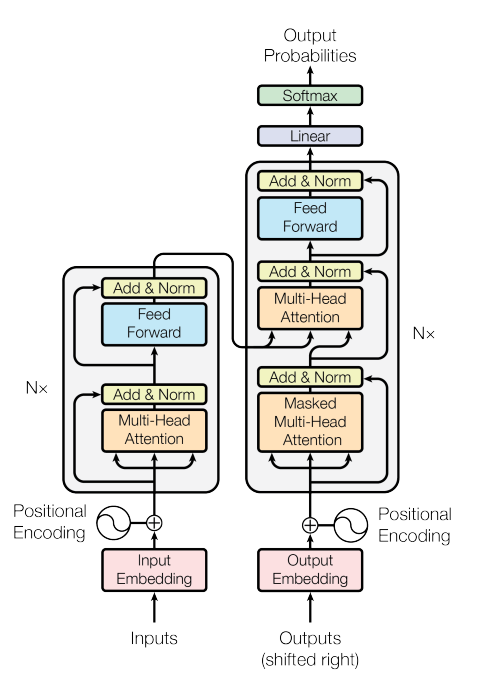
\includegraphics[width=0.8\linewidth]{capitulos/figuras/transformerarquitetura.png}
   \caption{Arquitetura apresenta por \textcite{https://doi.org/10.48550/arxiv.1706.03762}}
   \label{fig:arquitetura}
\end{figure}

A arquitetura do Transformer, baseada na estrutura de codificador-decodificador, desempenha um papel crucial no processamento eficiente de dados. O componente codificador transforma uma sequência de entrada em uma representação interna contínua, enquanto o decodificador utiliza essa representação para gerar a saída desejada de forma sequencial, com cada etapa autorregressiva usando as saídas anteriores como entrada adicional. Essa estrutura é complementada pelo mecanismo de autoatenção, que permite ao modelo capturar dependências de longo alcance de maneira eficaz. Diferentemente das redes neurais convolucionais (CNNs), que capturam características espaciais, ou das redes neurais recorrentes (RNNs), eficazes para dados sequenciais, os Transformers eliminam a necessidade dessas estruturas específicas, utilizando apenas camadas de atenção para lidar com a sequencialidade dos dados. Isso permite uma paralelização mais eficiente durante o treinamento e melhora a capacidade de modelar dependências de longo alcance \cite{THIRUNAVUKARASU2024100648}. 

A arquitetura do codificador-decodificador forma a base da transdução de sequência neuronal \cite{Vaswani2017}. O componente codificador do design converte uma sequência de representações de símbolos de entrada \(x_1, x_2, \ldots, x_n\) em uma sequência contínua \(z_1, z_2, \ldots, z_n\). O componente decodificador produz uma sequência de saída \(y_1, y_2, \ldots, y_m\), um de cada vez. Cada etapa autorregressiva usa os símbolos criados anteriormente como entrada adicional para criar a próxima. Existe uma estrutura de codificador/decodificador com auto-atenção em camadas e camadas ligadas pontualmente dentro do Transformer. A Figura \ref{fig:transformers} ilustra a arquitetura do Transformer mostrando o componente codificador que transforma a sequência de entrada em uma representação interna contínua, e o componente decodificador que gera a sequência de saída de forma sequencial.

\begin{figure}
    \centering
    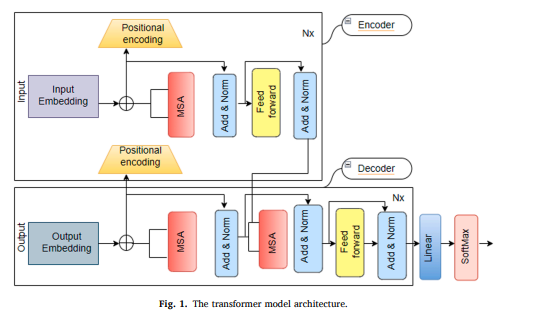
\includegraphics[width=1.0\linewidth]{capitulos//figuras/image_transformer.png}
    \caption{A arquitetura do Transformer codificados de \textcite{THIRUNAVUKARASU2024100648}}
    \label{fig:transformers}
\end{figure}


\textcite{LIN2022111} define a autoatenção como elemento central nas redes Transformers, tendo como objetivo eliminar a necessidade de estruturas recorrentes ou convolucionais, tradicionalmente empregadas para capturar relações temporais ou espaciais em dados sequenciais. A autoatenção confere aos modelos de rede Transformer a capacidade de atribuir diferentes níveis de importância às várias partes de uma sequência de entrada. Isso significa que, ao processar qualquer segmento da sequência, a rede pode efetivamente ponderar a importância em outros segmentos relevantes, identificando e realçando as conexões críticas entre eles. Esse processo não só enriquece a representação do contexto, mas também aprimora a capacidade da rede de interpretar e reagir a padrões complexos nos dados, tornando as redes Transformers extremamente eficazes em aplicações de processamento de linguagem natural e outras tarefas que exigem compreensão de sequências.

No contexto das redes Transformer, a autoatenção é um mecanismo essencial e pode ser descrito matematicamente através de três componentes principais: consultas (\(Q\)), chaves (\(K\)) e valores (\(V\)). Esses componentes são projetados a partir da entrada usando matrizes de pesos aprendidas. A autoatenção é calculada pela seguinte Equação \ref{eq:Attention}.

\begin{equation}
\text{Attention}(Q, K, V) = \text{softmax}\left(\frac{QK^T}{\sqrt{d_k}}\right)V
\label{eq:Attention}
\end{equation}

A Figura \ref{fig:etrans} ilustra o mecanismo de "scaled dot-product attention", onde as consultas (\(Q\)), chaves (\(K\)) e valores (\(V\)) são combinados para calcular a atenção de maneira escalonada, utilizando a divisão por \(\sqrt{d_k}\) para evitar valores extremamente grandes na função softmax, o que poderia levar a gradientes muito pequenos durante o treinamento.

\begin{figure}
    \centering
    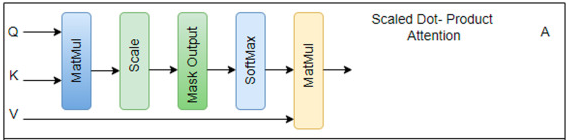
\includegraphics[width=1.0\linewidth]{capitulos//figuras/scalled.png}
    \caption{Mecanismo de atenção por produto escalar escalado (scaled dot-product attention), onde a função de atenção é aplicada utilizando consultas, chaves e valores escalonados.Figura de de \textcite{THIRUNAVUKARASU2024100648}}
    \label{fig:etrans}
\end{figure}

Em contraste com a aplicação de uma única função de atenção, as redes Transformer implementam a estratégia de atenção multi-cabeça. Neste mecanismo, as consultas, chaves e valores originais, que estão em uma dimensão \(d\), são projetados em novas dimensões \(d_q\), \(d_k\) e \(d_v\), respectivamente, usando \(h\) diferentes conjuntos de projeções aprendidas. Para cada um desses conjuntos, a saída é calculada utilizando a função de atenção. O modelo então concatena as saídas de cada uma das cabeças de atenção e as projeta de volta para uma representação unificada de dimensão \(d\), definido pela Equação \ref{eq:MultAttention}.

\begin{equation}
\begin{aligned}
\text{MultiHeadAttn}(Q, K, V) &= \text{Concat}(\text{head}_1, \ldots, \text{head}_h)W^O \\
\text{onde } \text{head}_i &= \text{Attention}(QW_i^{Q}, KW_i^{K}, VW_i^{V})
\label{eq:MultAttention}
\end{aligned}
\end{equation}

A Figura \ref{fig:enter-label} ilustra o mecanismo de "multi-head attention", mostrando como múltiplas cabeças de atenção operam em paralelo, permitindo que o modelo considere diferentes partes da entrada de diferentes maneiras, antes de combinar os resultados.

Na arquitetura do Transformer, existem três tipos de atenção:

1. Autoatenção: Utilizada no codificador Transformer, onde \(Q = K = V\), com \(Q\) representando as saídas da camada anterior.
   
2. Autoatenção mascarada: No decodificador Transformer, a autoatenção é limitada para que as consultas em cada posição só possam atender a posições até aquela específica. Isso é feito aplicando uma máscara à matriz de atenção não normalizada \(QK^T\).

3. Atenção cruzada: As consultas são projetadas a partir das saídas da última camada do decodificador, enquanto chaves e valores são projetados usando as saídas do codificador.

\begin{figure}
    \centering
    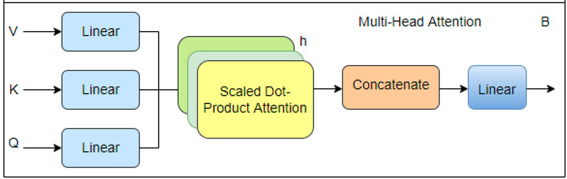
\includegraphics[width=1.0\linewidth]{capitulos//figuras/multi-head.png}
    \caption{Mecanismo de atenção multi-cabeça (multi-head attention), que permite que várias cabeças de atenção operem em paralelo, combinando suas saídas para uma representação final.Figura de de \textcite{THIRUNAVUKARASU2024100648}}
    \label{fig:enter-label}
\end{figure}

Entendendo o conceito geral das redes tranformers vamos apresentar o funcionamento de suas variantes como o Bert de \textcite{Develin}, Roberta de \textcite{Roberta}, Destilbert de \textcite{https://doi.org/10.48550/arxiv.1910.01108}, a Figura ~\ref{fig:linhatransformer} mostra a linha do tempo das arquiteturas transfomers.

\begin{figure}[H]
   \centering
   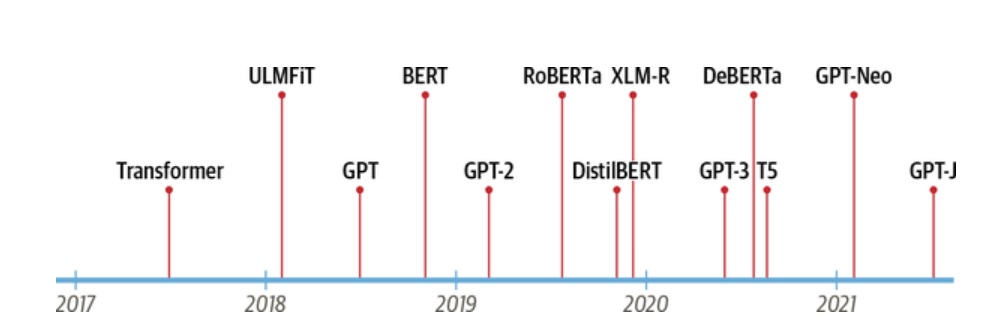
\includegraphics[width=0.8\linewidth]{capitulos/figuras/transformadoras.jpg}
   \caption{Linha do tempo apresentado por  \textcite{Tunstall2022-uq}}
   \label{fig:linhatransformer}
\end{figure}


O BERT (\textit{Bidirectional Encoder Representations from Transformers}) é um modelo de representação de linguagem baseado na arquitetura Transformer. No caso do BERT, durante o pré-treinamento, o modelo é exposto a grandes quantidades de texto não rotulado. Uma das técnicas utilizadas no pré-treinamento do BERT é o masked language modeling (MLM), onde palavras são aleatoriamente ocultadas em uma sequência de entrada e o modelo é treinado para prever as palavras ocultas com base no contexto das palavras circundantes. Isso permite ao BERT capturar o contexto bidirecional de cada palavra em uma frase, pois o modelo não apenas recebe informações de palavras anteriores, mas também de palavras subsequentes. O MLM é implementado aplicando uma máscara a algumas palavras de entrada e treinando o modelo para reconstruir essas palavras com base no contexto global da frase. Essa tarefa de reconstrução força o BERT a aprender representações ricas que capturam o significado das palavras e sua relação com o contexto \cite{Develin}.

Além do MLM, o BERT também emprega a técnica de Next sentence prediction (NSP) durante o pré-treinamento. A NSP envolve a tarefa de prever se uma frase é a próxima em um documento. Essa tarefa auxilia o modelo a capturar o contexto mais amplo de uma sequência de entrada, permitindo que ele entenda como as frases se relacionam umas com as outras. Dessa forma, o BERT aprende a capturar informações de contexto tanto em nível de palavra quanto em nível de frase, o que é crucial para muitas tarefas de processamento de linguagem natural.

Após o pré-treinamento, o BERT pode ser ajustado (fine-tuned) para tarefas específicas de linguagem natural, como classificação de texto, marcação de sequência e resposta a perguntas. Durante o ajuste fino, o modelo é treinado em um conjunto de dados rotulados relacionados à tarefa em questão. Os parâmetros do BERT são atualizados durante o treinamento, permitindo que o modelo se adapte à tarefa específica. Como o BERT já aprendeu representações ricas de linguagem durante o pré-treinamento, ele pode ser ajustado rapidamente para tarefas específicas, aproveitando o conhecimento prévio que adquiriu. Esse ajuste fino é essencial para adaptar o BERT a um domínio específico ou a uma tarefa específica, melhorando seu desempenho e capacidade de generalização.

O BERT se destaca por sua arquitetura unificada, que é aplicada de forma consistente em diferentes tarefas. Sua arquitetura é baseada em um codificador Transformer bidirecional com várias camadas, seguindo a implementação original proposta por \textcite{https://doi.org/10.48550/arxiv.1706.03762} e disponibilizada na biblioteca tensor2tensor. 

É importante ressaltar que, ao contrário do Transformer utilizado no GPT, o Transformer do BERT utiliza autoatenção bidirecional, permitindo que cada token considere o contexto tanto à sua esquerda quanto à sua direita \cite{Develin}. 


% 13 trabalho

No conjunto de estudos revisados, destaca-se o trabalho de \textcite{Reynald}, que utiliza redes transformers na abordagem UViT para estimar a fração de ejeção ventricular esquerda (FEVE) em fluxos de vídeo de ecocardiograma. O modelo UVT (Ultrasound Video Transformer) opera em duas etapas: primeiro, uma rede neural convolucional (ResNetAE) extrai características dos quadros de vídeo de ecocardiografia. Em seguida, um transformador inspirado na arquitetura BERT processa essas características para prever a FEVE, capturando relações temporais entre os quadros. A UViT apresentou um MAE (Erro Médio Absoluto) de 5,95 e R² de 0,52 no conjunto de dados EchoNet-Dynamic, superando o desempenho de outros métodos de aprendizado profundo.

A arquitetura UViT proposta inclui três módulos: um codificador para reduzir a dimensionalidade dos dados, um módulo BERT para raciocínio espaço-temporal, e dois regressores para prever os índices dos quadros de fim de sístole (ES) e fim de diástole (ED), além da FEVE. Na redução da dimensionalidade, um ResNetAE destila os quadros de ultrassom em vetores de 1024 dimensões, que são empilhados formando a incorporação inicial do vídeo (Lote x Quadros x 1024). Esta incorporação é então processada pelo modelo transformer, treinado de ponta a ponta, otimizando o desempenho em tarefas de interpretação de ultrassom cardíaco.

Para capturar relações espaciais-temporais, um encoder BERT é utilizado com uma rede de regressão, formando um modelo de Reconhecimento de Entidades Nomeadas (NER). As incorporações extraídas do ResNetAE são usadas como entrada para o encoder BERT, que contém blocos de autoatenção e atenção, regularizados por camadas de dropout. Após a extração das informações espaciais-temporais pelos encoders BERT e ResNetAE, as características combinadas formam um vetor final, utilizado por dois regressores. O primeiro prevê os índices dos quadros de fim de sístole (ES) e fim de diástole (ED), enquanto o segundo estima a FEVE. Durante o treinamento do regressor da FEVE, são utilizadas perdas combinadas e técnicas de regularização para lidar com o desequilíbrio na distribuição dos valores de FEVE no conjunto de treinamento. A Figura ~\ref{fig:reynaldarq} apresenta uma visão geral da arquitetura proposta para a predição da FEVE em vídeos de ultrassom cardíaco. A operação @ representa o produto escalar entre vetores. Essa arquitetura integrada permite a combinação das informações extraídas de diferentes etapas para uma melhor predição da FEVE em vídeos de ultrassom cardíaco.

\begin{figure}[!ht]
   \centering
   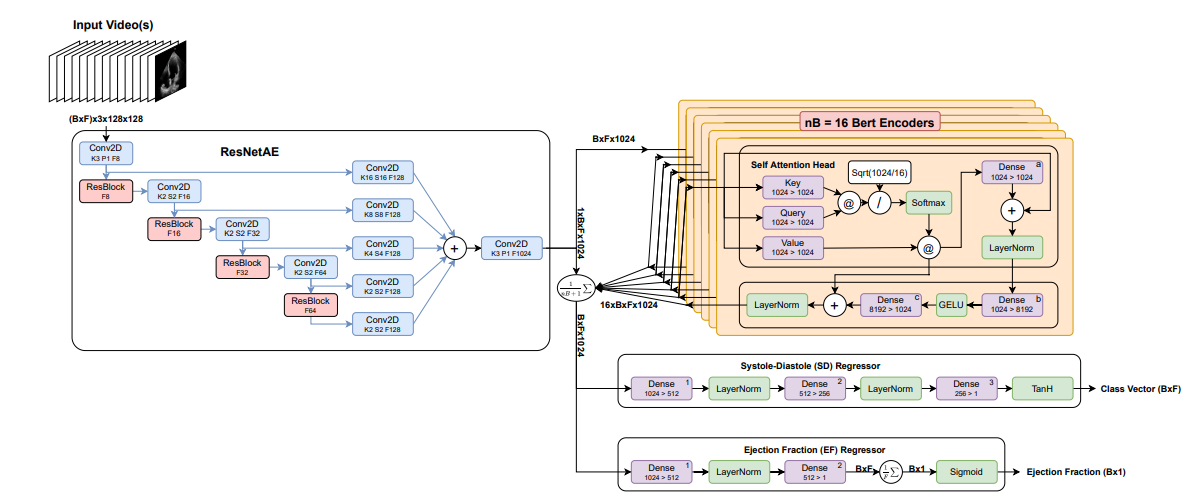
\includegraphics[width=1.0\linewidth]{capitulos/figuras/reynald.png}
   \caption{A Figura apresenta uma visão geral da arquitetura proposta por \textcite{Reynald}.}
   \label{fig:reynaldarq}
\end{figure}

\section{Análise de trabalhos potenciais}
\label{Avaliação de trabalhos potenciais}

Durante a fase inicial de nossa investigação, conduzimos uma revisão sistemática da literatura sobre os métodos predominantes empregados na análise de ecocardiogramas utilizando técnicas de inteligência artificial. Observou-se que a maioria dos estudos recentes recorre predominantemente a redes neurais convolucionais (CNNs). A aplicação  dessas redes foi consistentemente destacada em nossa revisão sistemática da literatura. No entanto, notamos que as melhorias proporcionadas por essas técnicas podem estar se aproximando de um platô em termos de inovação. Esta tendência demonstra a necessidade de explorar novas abordagens tecnológicas para avançar além dos limites atuais.

Especificamente, estudos exemplares como os realizados por \textcite{LIU2021101873}, \textcite{9648607}, e \textcite{9335592}, que utilizam CNNs na análise de ecocardiogramas, com foco em segmentação de imagem e detecção de características cardíacas, confirmam essa observação. Embora esses estudos tenham conseguido avanços significativos, a repetição de abordagens similares e a dependência de incrementos finos na precisão e eficiência podem indicar uma certa maturidade da tecnologia que limita saltos de inovação. Este cenário reflete as conclusões de nossa revisão sistemática, destacando a necessidade de abordagens novas para impulsionar o campo da análise de ecocardiogramas por inteligencia artificial.

A revisão sistemática da literatura revelou que, apesar do vasto número de aplicações, há uma lacuna notável no aproveitamento de tecnologias emergentes como as redes Transformers, que oferecem novas perspectivas para o processamento de dados médicos de imagem. A arquitetura UViT, desenvolvida por \textcite{Reynald}, por exemplo, se destacou pela integração de elementos dos modelos Transformer para analisar sequências de imagens temporais — uma abordagem ainda pouco explorada em ecocardiogramas.

\textcite{Atabansi2023} sugere que os avanços arquiteturais recentes em redes Transformer poderiam oferecer uma nova direção para superar os limites observados com as CNNs, possibilitando uma captura mais eficaz de dinâmicas espaço-temporais complexas, que são cruciais em diagnósticos médicos. Diante deste contexto, propomos adotar e evoluir a arquitetura UViT para analisar ecocardiogramas em nosso trabalho, justificada pela habilidade superior das redes transformadoras de processar sequências de dados complexas. As redes convencionais, embora eficazes em muitas aplicações médicas, apresentam limitações na análise de sequências temporais e na compreensão de contextos mais amplos nas imagens. A arquitetura UViT, que integra elementos de redes Transformer, é particularmente promissora para superar essas limitações. Sua estrutura é desenhada para processar dados não só em um contexto espacial — como é típico nas CNNs — mas também em um contexto temporal, fazendo uso eficiente da autoatenção para entender a relação entre frames sequenciais de um ecocardiograma. Essa capacidade de perceber e integrar informações ao longo do tempo permite uma representação mais rica e detalhada do coração em movimento, potencializando a precisão diagnóstica.

A lacuna atual na aplicação da arquitetura UViT em ecocardiogramas oferece uma oportunidade significativa de inovação. Planejamos implementar e aprimorar a UViT em nossa pesquisa, integrando avanços recentes em técnicas de autoatenção, como RoBERTa e DistilBERT. Essa integração visa refinar a capacidade da rede de processar informações complexas e volumosas, com um foco especial em melhorar a precisão na previsão da fração de ejeção do coração. Além disso, pretendemos expandir a aplicação da UViT para incluir dados de pacientes adultos e pediátricos. Uma explicação  desta estratégia  será apresentada no Capítulo \ref{Metodologia}. 

